\documentclass[12pt, titlepage]{article}

\usepackage{fullpage}
\usepackage[round]{natbib}
\usepackage{multirow}
\usepackage{booktabs}
\usepackage{tabularx}
\usepackage{graphicx}
\usepackage{float}
\usepackage{hyperref}
\hypersetup{
    colorlinks,
    citecolor=black,
    filecolor=black,
    linkcolor=red,
    urlcolor=blue
}
\usepackage[round]{natbib}

\newcounter{acnum}
\newcommand{\actheacnum}{AC\theacnum}
\newcommand{\acref}[1]{AC\ref{#1}}

\newcounter{ucnum}
\newcommand{\uctheucnum}{UC\theucnum}
\newcommand{\uref}[1]{UC\ref{#1}}

\newcounter{mnum}
\newcommand{\mthemnum}{M\themnum}
\newcommand{\mref}[1]{M\ref{#1}}

\title{SE 3XA3: Software Requirements Specification\\QChat}

\author{Team \#14, QChat
		\\ Adit Patel - patela14
		\\ Harsh Patel - patelh11
		\\ Vrushesh Patel - patelv12
}

\date{November 10, 2017}

% \input{../../Comments}

\begin{document}

\maketitle

\pagenumbering{roman}
\tableofcontents
\listoftables
\listoffigures

\begin{table}[h!]
\caption{\bf Revision History}
\begin{tabularx}{\textwidth}{p{3cm}p{2cm}X}
\toprule {\bf Date} & {\bf Version} & {\bf Notes}\\
\midrule
10/11/2017 & 1 & Initial Version\\
25/11/2017 & 2 & Updated Module Decomposition - Software Decision \\
06/12/2017 & Rev 1.0 & Final Revision \\
\bottomrule
\end{tabularx}
\end{table}

\newpage

\pagenumbering{arabic}
\newpage
\section{Introduction}


This document indicates the Module Guide for the implementation of the QChat anonymous questions and answers web app. This document is intended to facilitate the design and maintenance of the project while giving and through and clear specifications of the interfacing that occurs between the different modules in the project.\\

One common approach to developing software that is commonly accepted is decomposing the system into modules and then interconnecting them in way that allows for the system to be easily maintained and updated. Any work assignment for a programmer or a programming team is considered to be a module. This module guide will allows for designers and maintainers to easily identify different parts of the software. \\
 
Our system design will follow the following rules:
\begin{itemize}
\item Each module will be designed to handle a specific task
\item System details that are handled independently should be secrets of separate modules, this is where information hiding will be used.
\item Other programs/modules that require information stored in a certain module’s data must obtain it by calling access programs that belong to that module.
\end{itemize}

The potential readers of this document are one or more of the following:
\begin{itemize}
\item \textbf{New Project Members:} Any new member to the team will be expected to read this document to understand the structure of the project and how the different modules interact to make  the system work. Reading this document will also answer most trivial questions a new member will have regarding the project.
\item \textbf{Project Maintainers:} The software maintenance team will be expected to read this document as it will give them a good understanding of the hierarchical structure of the modules and how they are prioritized and interconnected. 
\item \textbf{Project Designers:} Designers can use this document to check for consistency, feasibility and flexibility of the system. Designers can use many techniques to verify the system however they must all match the expected results noted and implied in this document.
\end{itemize}

\section{Anticipated and Unlikely Changes} \label{SecChange}

This section lists possible changes to the system. According to the likeliness
of the change, the possible changes are classified into two
categories. Anticipated changes are listed in Section \ref{SecAchange}, and
unlikely changes are listed in Section \ref{SecUchange}.

\subsection{Anticipated Changes} \label{SecAchange}

Anticipated changes are the source of the information that is to be hidden
inside the modules. Ideally, changing one of the anticipated changes will only
require changing the one module that hides the associated decision. The approach
adapted here is called design for
change.

\begin{description}
\item[\refstepcounter{acnum} \actheacnum \label{acHardware}:] The hardware on which the application is going to run.
\item[\refstepcounter{acnum} \actheacnum \label{ac2}:] The database used by the application.
\item[\refstepcounter{acnum} \actheacnum \label{ac3}:] The format of input data (eg. SessionID could be changed to take only numbers).
\item[\refstepcounter{acnum} \actheacnum \label{ac4}:] The user interface of the application.
\item[\refstepcounter{acnum} \actheacnum \label{ac5}:] Adding feature to trace the user from their posts while keeping it anonymous (can only be used by authorized person).
\end{description}

\subsection{Unlikely Changes} \label{SecUchange}

The module design should be as general as possible. However, a general system is
more complex. Sometimes this complexity is not necessary. Fixing some design
decisions at the system architecture stage can simplify the software design. If
these decision should later need to be changed, then many parts of the design
will potentially need to be modified. Hence, it is not intended that these
decisions will be changed.

\begin{description}
\item[\refstepcounter{ucnum} \uctheucnum \label{ucIO}:] The format of the data stored (eg. JSON).
\item[\refstepcounter{ucnum} \uctheucnum \label{ucInput}:] The goal of the application: To allow users to ask questions and reply answers anonymously.
\item[\refstepcounter{ucnum} \uctheucnum \label{ucInput}:] The web technologies used to make QChat.
\item[\refstepcounter{ucnum} \uctheucnum \label{ucInput}:] The structure of the data stored.
\item[\refstepcounter{ucnum} \uctheucnum \label{ucInput}:] Firebase configuration data (eg. API key, database URL).
\end{description}

\section{Module Hierarchy} \label{SecMH}

This section provides an overview of the module design. Modules are summarized
in a hierarchy decomposed by secrets in Table \ref{TblMH}. The modules listed
below, which are leaves in the hierarchy tree, are the modules that will
actually be implemented.

\begin{description}
\item [\refstepcounter{mnum} \mthemnum \label{mHH}:] Hardware-Hiding Module
\item [\refstepcounter{mnum} \mthemnum \label{mDM}:] Data Manipulation Module
\item [\refstepcounter{mnum} \mthemnum \label{mIF}:] Initializer/Firebase Module
\item [\refstepcounter{mnum} \mthemnum \label{mUI}:] UI Module
\item [\refstepcounter{mnum} \mthemnum \label{mCS}:] Client/Server Communication Module
\item [\refstepcounter{mnum} \mthemnum \label{mIV}:] Input verification Module
\end{description}


\begin{table}[h!]
\centering
\begin{tabular}{p{0.33\textwidth} p{0.33\textwidth} p{0.33\textwidth}}
\toprule
\textbf{Level 1} & \textbf{Level 2} (Model) & \textbf{Level 3} (View/Controller)\\
\midrule

{Hardware-Hiding Module} & ~ \\
\midrule

\multirow{7}{0.3\textwidth}{Behaviour-Hiding Module} & ~ \\
& Data Manipulation Module & UI Module \\ & & Client/Server Communication Module \\
\midrule

\multirow{3}{0.3\textwidth}{Software Decision Module}\\
& Initializer/Firebase Module & Input verification Module  \\
\bottomrule

\end{tabular}
\caption{Module Hierarchy}
\label{TblMH}
\end{table}

\section{Connection Between Requirements and Design} \label{SecConnection}

The design of the system is intended to satisfy the requirements developed in
the SRS. In this stage, the system is decomposed into modules. The connection
between requirements and modules is listed in Table \ref{TblRT}.

\section{Module Decomposition} \label{SecMD}

Modules are decomposed according to the principle of ``information hiding''
proposed by \citet{ParnasEtAl1984}. The \emph{Secrets} field in a module
decomposition is a brief statement of the design decision hidden by the
module. The \emph{Services} field specifies \emph{what} the module will do
without documenting \emph{how} to do it. For each module, a suggestion for the
implementing software is given under the \emph{Implemented By} title. If the
entry is \emph{OS}, this means that the module is provided by the operating
system or by standard programming language libraries.  Also indicate if the
module will be implemented specifically for the software.

Only the leaf modules in the
hierarchy have to be implemented. If a dash (\emph{--}) is shown, this means
that the module is not a leaf and will not have to be implemented. Whether or
not this module is implemented depends on the programming language
selected.

\subsection{Hardware Hiding Modules (\mref{mHH})}

\begin{description}
\item[Secrets:]Although there isn't any physical hardware involved for our project, the data structures and algorithms used to implement the virtual hardware are the secrets of this module.
\item[Services:]Serves as virtual hardware used by the rest of the system, this module provides the interface between the hardware and the software which will allow the system to use it to display outputs and accept inputs.
\item[Implemented By:] OS
\end{description}

\subsection{Behaviour-Hiding Module}

\begin{description}
\item[Secrets:]The contents of the required behaviours.
\item[Services:]Includes programs that provide externally visible behaviour of
  the system as specified in the software requirements specification (SRS)
  documents. This module serves as a communication layer between the
  hardware-hiding module and the software decision module. The programs in this
  module will need to change if there are changes in the SRS.
\item[Implemented By:] --
\end{description}


\subsubsection{Data Manipulation Module (\mref{mDM})}
\begin{description}
\item[Secrets:]How to manipulate/store/access/update data and where it is placed and accessed.
\item[Services:]Updates database, fetches data and returns it to the accessing module.
\item[Implemented By:] -
\end{description}


\subsubsection{User Interface Module (\mref{mUI})}
\begin{description}
\item[Secrets:]UI features implementation, how it's updated dynamically.
\item[Services:]Updated UI as user interacts with the different fields available, shows data.
\item[Implemented By:]Html files, CS files and JavaScript files
\end{description}


\subsubsection{Client/Server Communication Module (\mref{mCS})}
\begin{description}
\item[Secrets:]How and where communication occurs
\item[Services:]Transferring data from other module to database and accessing data from database to use in other modules
\item[Implemented By:]Index.js file, Firebase
\end{description}






\subsection{Software Decision Module}

\begin{description}
\item[Secrets:] The design decision based on mathematical theorems, physical
  facts, or programming considerations. The secrets of this module are
  \emph{not} described in the SRS.
\item[Services:] Includes data structure and algorithms used in the system that
  do not provide direct interaction with the user. 
  % Changes in these modules are more likely to be motivated by a desire to
  % improve performance than by externally imposed changes.
\item[Implemented By:] --
\end{description}

\subsubsection{Client/Server Communication Module (\mref{mIV})}
\begin{description}
\item[Secrets:]How inputted data is verified is hidden from other modules.
\item[Services:]Handles user inputs, checks for correct input semantics before packaging and transferring inputted data to other modules
\item[Implemented By:]Index.js file, Html files, CS files and JavaScript files, Firebase
\end{description}


\section{Traceability Matrix} \label{SecTM}

This section shows two traceability matrices: between the modules and the
requirements and between the modules and the anticipated changes.

% the table should use mref, the requirements should be named, use something
% like fref
\begin{table}[H]
\centering
\begin{tabular}{p{0.4\textwidth} p{0.6\textwidth}}
\toprule
\textbf{Req.} & \textbf{Modules}\\
\midrule
Functional - 1 & \mref{mHH}, \mref{mDM}, \mref{mIF}, \mref{mUI}, \mref{mCS}, \mref{mIV} \\
Functional - 2 & \mref{mHH}, \mref{mDM}, \mref{mIF}, \mref{mUI}, \mref{mCS}, \mref{mIV}\\
Functional - 3 & \mref{mUI}, \mref{mCS}, \mref{mIV} \\
Functional - 4 & \mref{mDM}, \mref{mUI}, \mref{mIV}\\
Non-Functional-3.1 & \mref{mUI}\\
Non-Functional-3.2 & \mref{mUI}, \mref{mIV}\\
Non-Functional-3.3 & \mref{mDM}, \mref{mIF}, \mref{mUI}, \mref{mCS}, \mref{mIV}\\
Non-Functional-3.4 & \mref{mIF}, \mref{mCS}, \mref{mIV}\\
Non-Functional-3.5 & \mref{mDM}, \mref{mIF}, \mref{mCS}\\
Non-Functional-3.6 & \mref{mDM}, \mref{mIF}, \mref{mCS}\\
Non-Functional-3.7 & \mref{mDM}, \mref{mUI}, \mref{mIV}\\
\bottomrule
\end{tabular}
\caption{Trace Between Requirements and Modules}
\label{TblRT}
\end{table}

\begin{table}[H]
\centering
\begin{tabular}{p{0.2\textwidth} p{0.6\textwidth}}
\toprule
\textbf{AC} & \textbf{Modules}\\
\midrule
\acref{acHardware} & \mref{mHH}\\
\acref{ac2} & \mref{mIF}, \mref{mCS}\\
\acref{ac3} & \mref{mIV}\\
\acref{ac4} & \mref{mUI}\\
\acref{ac5} & \mref{mDM}, \mref{mIF}, \mref{mCS}, \mref{mIV}\\

\bottomrule
\end{tabular}
\caption{Trace Between Anticipated Changes and Modules}
\label{TblACT}
\end{table}

\section{Use Hierarchy Between Modules} \label{SecUse}



\begin{figure}[H]
\centering
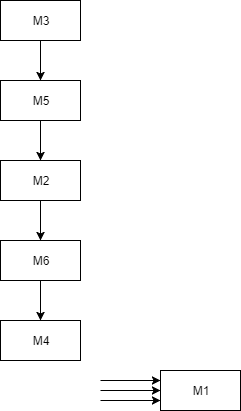
\includegraphics[width=0.5\textwidth]{UsesHierarchy.png}
\caption{Use hierarchy among modules}
\label{FigUH}
\end{figure}

%\section*{References}

\bibliographystyle {plainnat}
\bibliography {MG}

\end{document}
